% !TEX root = ../main.tex
\chapter{Constraints on configurations}\label{ch:c16}
\begin{paracol}{2}

\begin{sources}
\begin{tabularx}{\linewidth}{@{}l l L@{}}
\toprule
\textbf{Video} & \textbf{Length} & \textbf{Content}\\
\midrule
\seg{16}{1}{Lecture 16: Constraints on configurations (Zwangsbedingungen an Konfigurationen)} & 1:37:36 & The promise of the double pendulum; recall of the Lagrangian of one and of $N$ particles; holonomic constraints as a smooth submanifold of the configuration space, embedded by an injective smooth map $h$; why injectivity; the Lagrangian of the constrained system as $L\circ h_*$; the linear push-forward of vectors, defined by its action on functions, with the curve picture; its components in charts; the recipe of modelling; the Lagrangian of an uncharged particle under constraints and the induced metric; a question on the foot point of $h_*X$. The recorded date is 17 June 2014.\\
\bottomrule
\end{tabularx}

\smallskip
\textbf{Transcript} \file{materials/transcripts/C16-V01.txt} (German YouTube auto-captions, mediocre in the spoken formulas; the formulas are reconstructed by recomputing and marked [?] where unsure).
\end{sources}

\begin{reading}[Where this lecture sits in the other notes]
Not treated in the other courses.
Continues \cref{ch:c15} (configuration space of $N$ particles); the next lecture, \cref{ch:c17}, turns the construction into a five-step algorithm and applies it to the pendulum and the double pendulum.
\end{reading}

% ==================================================================
\section{The promise: mechanical systems with constraints}\label{sec:zw-promise}

Schuller is back (the lecture is his; the previous one was given by his substitute, \cref{ch:c15}). Today he keeps his promise: ``we will understand how to treat mechanical systems that are subject to \emph{constraints} (Zwangsbedingungen)'', as for instance the \emph{double pendulum} \ts{16}{1}{0:04}. It is a mechanical system of two particles, but the two particles do not move freely in absolute space (that was last time: the Lagrangian of two free particles). Now we \emph{add constraints}: the first particle is forced to keep a constant distance from the suspension point (a pendulum rod), the second is forced to keep a constant distance from the first (another rod) \ts{16}{1}{0:25}.

\begin{nfigure}
\begin{tikzpicture}[scale=0.85]
  % allowed
  \begin{scope}
    \fill (0,0) circle (2pt); \draw[thick] (-0.4,0) -- (0.4,0);
    \draw[thick] (0,0) -- (1.1,-1.5) coordinate (A);
    \draw[thick] (A) -- (2.5,-3.0) coordinate (B);
    \fill[blue!70!black] (A) circle (3pt); \fill[red!70!black] (B) circle (3pt);
    \node at (1.2,-3.9) {allowed configuration};
  \end{scope}
  \begin{scope}[xshift=7cm]
    \fill (0,0) circle (2pt); \draw[thick] (-0.4,0) -- (0.4,0);
    \draw[thick] (0,0) -- (-1.1,-1.5) coordinate (A);
    \draw[thick] (A) -- (0.9,-3.1) coordinate (B);
    \fill[blue!70!black] (A) circle (3pt); \fill[red!70!black] (B) circle (3pt);
    \node at (0,-3.9) {another allowed configuration};
  \end{scope}
  \begin{scope}[xshift=14cm]
    \fill (0,0) circle (2pt); \draw[thick] (-0.4,0) -- (0.4,0);
    \draw[dashed,gray] (0,0) circle (1.85);
    \fill[blue!70!black] (-1.7,-0.8) circle (3pt); \fill[red!70!black] (2.3,-2.4) circle (3pt);
    \node at (0.2,-3.9) {\textbf{not} allowed};
  \end{scope}
\end{tikzpicture}
\caption*{The planar double pendulum: two allowed configurations of the two masses, and a configuration of absolute space which does not satisfy the two constraints (each mass at a wrong distance from its rod's end).}
\end{nfigure}
The positions of the two particles in the first picture form an \emph{allowed configuration} in the presence of the constraints; another allowed configuration is the second position; \emph{not} allowed would be, for instance, one particle here and the other there: it is a configuration in absolute space, but it does not agree with the two constraints \ts{16}{1}{1:06}--\ts{16}{1}{1:27}. Today we see how to describe this theoretically.

% ==================================================================
\section{Recall}\label{sec:zw-recall}

\begin{recall}[One particle, $N$ particles (\cref{ch:c13,ch:c14,ch:c15})]\label{rec:zw-recall}
\emph{One particle} (two lectures ago): the world path $\sigma\colon\R\to\mathcal R$ (he now calls the curve $\sigma$, before $\gamma$) into absolute space; the \emph{lifted} curve $\tilde\sigma$ lives in the tangent bundle $T\mathcal R$, the velocity phase space. The Lagrangian of a system is always a smooth real function on the velocity phase space of the space underlying the system, $L\colon T\mathcal R\to\R$, and the action is $S[\sigma]=\int_a^b\mathrm d\lambda\,L(\tilde\sigma(\lambda))$; for a suitable $L$ it encodes the whole dynamics, since the stationary curves are the paths the particle follows. The Euler--Lagrange equations (\cref{thm:var-el}) follow from the stationarity; the whole construction has nothing to do with coordinates, but to \emph{compute} one goes into a chart $x$ of the absolute space, with its induced chart $\xi_x$ of $T\mathcal R$ (\cref{def:lag-xi}); then, with $d=\dim\mathcal R$ ($=3$),
\[
  \frac{\mathrm d}{\mathrm d\lambda}\Bigl(\partial_{d+j}L_{(x)}\bigl(\xi_x\circ\tilde\sigma(\lambda)\bigr)\Bigr)-\partial_jL_{(x)}\bigl(\xi_x\circ\tilde\sigma(\lambda)\bigr)=0,\qquad j=1,\dots,d,
\]
where one first differentiates with respect to the entries and \emph{then} inserts the lifted curve \ts{16}{1}{1:48}--\ts{16}{1}{6:20}.

\emph{$N$ particles} (last lecture, \cref{ch:c15}): not $N$ curves but \emph{one} curve $\Sigma(\lambda)=(\sigma_1(\lambda),\dots,\sigma_N(\lambda))$ in the \emph{configuration space} $\mathcal Q=\mathcal R^N$ (the $N$-fold Cartesian product of absolute space; a photograph of the particles at one instant is $N$ points of $\mathcal R$, which is \emph{one} point of $\mathcal Q$), and the individual curves are recovered by the projections, $\sigma_j=\mathrm{pr}_j\circ\Sigma$ (\cref{eq:mp-Gamma,eq:mp-proj}) \ts{16}{1}{6:40}--\ts{16}{1}{11:53}. The smooth structure of $\mathcal Q$ is inherited: from charts $x_j$ of $\mathcal R$ one builds the product charts $\omega$ of $\mathcal Q$ (\cref{def:mp-omega}), and from the $\omega$ the induced charts of $T\mathcal Q$. From there on, mechanics runs \emph{as before}: a Lagrangian $L\colon T\mathcal Q\to\R$, the lifted curve $\tilde\Sigma$ in $T\mathcal Q$, the action $S[\Sigma]=\int\mathrm d\lambda\,L(\tilde\Sigma(\lambda))$ and the Euler--Lagrange equations: one for every coordinate of $\mathcal Q$, i.e.\ $Nd$ of them \ts{16}{1}{11:53}--\ts{16}{1}{14:58}.
\end{recall}

\begin{coursenote}[A correction on the index range (as said in class)]\label{cn:zw-index}
Writing the Euler--Lagrange equations for the chart built from $\omega$, Schuller first writes the derivative in the second slot as the $j$-th derivative with respect to $\dot{}$-entries; a student points out that the tangent bundle $T\mathcal Q$ has dimension $2Nd$ and the velocity entries come \emph{after} the $Nd$ position entries. He agrees: the derivative of the velocity entries is $\partial_{Nd+j}$ (and the second term $\partial_j$), with $j=1,\dots,Nd$; ``so many equations we must have: one particle in $d$ dimensions has $d$ equations, now we have $N$ times as many'' \ts{16}{1}{14:58}--\ts{16}{1}{16:01}.
\end{coursenote}

Does one really have to go from absolute space to the configuration space, and then again to the velocity phase space \emph{of the configuration space}? Yes: that is the successive construction of charts. After some practice one just ``has'' the configuration space in the pocket and does not rebuild it each time, but if one really treats $N$ particles in absolute space, this is how it is built, and it settles a hundred thousand unclear things which then follow from it. Schuller may arrange a question session, since last Thursday he himself could not be there \ts{16}{1}{16:01}--\ts{16}{1}{17:24}.

% ==================================================================
\section{Holonomic constraints on configurations}\label{sec:zw-holo}

Today's first section: \textbf{holonomic constraints (holonome Zwangsbedingungen) on the configurations} \ts{16}{1}{17:24}. The constraints are imposed neither on absolute space nor on the velocities, but on the \emph{configurations}.

\begin{coursenote}[The word ``holonomic'' (not said in class)]\label{cn:zw-holonomic}
The adjective is Greek: \emph{holos} ``whole'' and \emph{nomos} ``law'' (the constraint is a ``whole law'' on the positions alone, in contrast to constraints on the velocities). Schuller does not comment on the word.
\end{coursenote}

The basic idea, put into words: we want to consider systems whose configuration space is \emph{wilfully} (``mutwillig'': there is no reason for it except that we want it) \textbf{restricted to a smooth submanifold} \ts{16}{1}{17:47}--\ts{16}{1}{18:33}. What that means one sees in the double pendulum picture: why are the allowed configurations a smooth submanifold, when the picture is only two-dimensional? Absolute space is (in the picture) two-dimensional, there are two particles; the dimension of the configuration space $\mathcal Q$ is $2\cdot2=4$. One cannot draw a nice picture, but one can think: all configurations that the double pendulum allows lie in the four-dimensional space as a smooth submanifold. If one discussed the pendulum in \emph{absolute} space instead of in its configuration space, it would be a mess: all the points where the particles can be keep overlapping and crossing one another; lifted to the four-dimensional configuration space the allowed set is a perfectly smooth submanifold, and one can work with that \ts{16}{1}{18:33}--\ts{16}{1}{19:57}.

\begin{example}[Examples of holonomic constraints, and one which is not]\label{ex:zw-examples}
Pendulums, of course. A train on \emph{rails} (it may move on the earth surface in one direction only, instead of two); how would the train move on the rails, if the rails go around a curve? what is the dynamics? An arm \emph{in plaster} (``Gipsarm''): the configuration space is restricted, one cannot scratch one's nose with it any more. A dog on a \emph{leash}: it can run away only as far as the leash is long, but it can also come closer, and then the leash sags; that is \textbf{not} a holonomic constraint (``it exists for children as well''), because the region the dog or child can reach is not a submanifold, certainly not one of reduced dimension \ts{16}{1}{19:57}--\ts{16}{1}{21:21}.
\end{example}

\begin{definition}[New concepts: accessible configurations; holonomic constraints]\label{def:zw-access}
Let $\mathcal Q$ be the configuration space of the system \emph{without} constraints. The \textbf{accessible configurations (zug\"angliche Konfigurationen)} are a subset
\[
  \mathcal Z\ \subseteq\ \mathcal Q
\]
of all possible configurations (the two masses of the double pendulum cannot be anywhere, because of the rods) which forms a smooth \textbf{submanifold} of $\mathcal Q$ of dimension $\dim\mathcal Q-f$; here $f$ is the number of holonomic constraints (``anzahl der holonomen zwangsbedingungen''), and a submanifold is a subset which is itself a manifold, i.e.\ it has a smooth atlas \ts{16}{1}{21:21}--\ts{16}{1}{22:45}. Such constraints are called \textbf{holonomic} \ts{16}{1}{22:04}.
\end{definition}

\begin{coursenote}[$f$ is used for two different numbers (as said in class)]\label{cn:zw-f}
At \ts{16}{1}{22:04} $f$ is the \emph{number of constraints}, so that $\dim\mathcal Z=\dim\mathcal Q-f$. Later in the same lecture the same letter is used for the \emph{dimension} of $\mathcal Z$ (its charts are said to go into $\R^f$, \ts{16}{1}{56:14}) and Schuller half corrects himself (``here it should be the dimension of $\mathcal Z$'', \ts{16}{1}{1:21:53}). In these notes: $D:=\dim\mathcal Q$ ($=Nd$), $n:=\dim\mathcal Z$ and $f=D-n$ the number of constraints; the next lecture uses the letter $f$ for $\dim\mathcal Z$ (\cref{cn:pc-f}).
\end{coursenote}

Picture, for one particle in two dimensions (there the configuration space is the absolute space itself): a simple pendulum has as possible places only the points of a circle; the whole absolute space is $\mathcal Q$ (two-dimensional), the circle is $\mathcal Z\subset\mathcal Q$, and it can be drawn in the same space \ts{16}{1}{22:45}--\ts{16}{1}{23:49}. But how long is the pendulum rod? The pendulum can swing around a whole circle, so $\mathcal Z$ is the manifold $S^1$; but there can be a small $S^1$ or a big one, depending on the rod; one wants to know exactly \emph{how the circle is embedded}. That is the precise \emph{position} of $\mathcal Z$ in $\mathcal Q$ \ts{16}{1}{23:49}--\ts{16}{1}{24:54}.

\begin{definition}[New concepts: the embedding $h$ of the constraint]\label{def:zw-h}
The precise position of $\mathcal Z$ in $\mathcal Q$ is encoded, or given, by an \textbf{injective smooth map}
\[
  h\colon\mathcal Z\to\mathcal Q ,
\]
which says which point of $\mathcal Z$ is mapped onto which point of $\mathcal Q$ \ts{16}{1}{24:54}--\ts{16}{1}{25:14}. (Physically: if I say my forearm is a pendulum, I can give the angle of the elbow as a parameter, and say: at this angle the hand lies at this point of space; with a shorter arm it would be another map.) Which accessible configurations one has, and which $h$ one uses, one \emph{gives}; how, depends on the physical problem and on how one models it \ts{16}{1}{25:14}--\ts{16}{1}{25:57}.
\end{definition}

\emph{Why injective?} Suppose $\mathcal Z$ is mapped into $\mathcal Q$ so that the image crosses itself, like a figure eight: the same point of $\mathcal Q$ is hit by two different points of the circle. Then the circle itself is a manifold, but if one restricted the system to that image, the particle running along it would at the crossing either slide on to one branch or to the other, and \emph{one would not have this under control}. Such a thing would no longer be a holonomic constraint, and it is excluded: this is the philosophical reason for describing constraints by submanifolds embedded by an injective map; ``it will become technically important in a moment'' \ts{16}{1}{25:57}--\ts{16}{1}{27:20}.

\begin{nfigure}
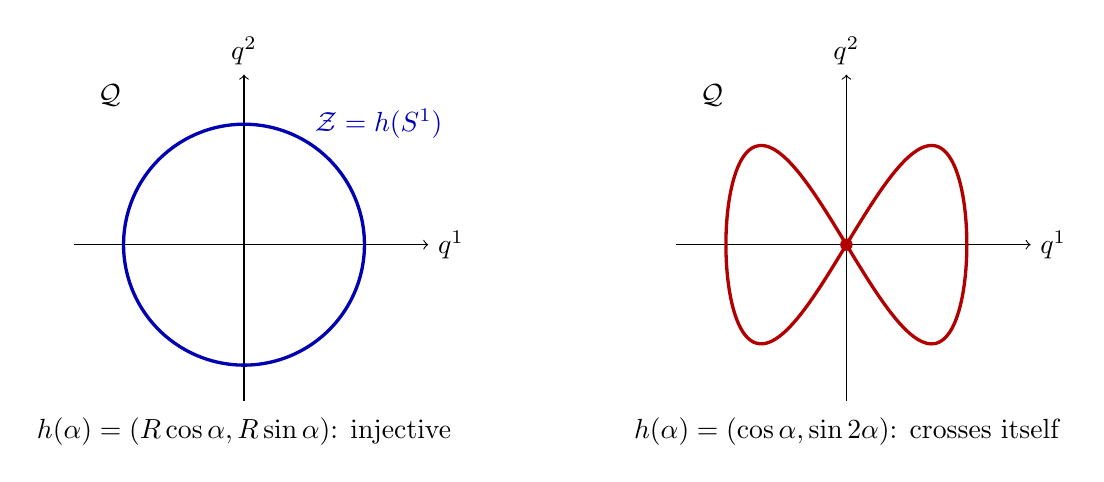
\begin{tikzpicture}[scale=0.9]
  \begin{scope}
    \draw[->] (-2.4,0) -- (2.6,0) node[right] {$q^1$}; \draw[->] (0,-2.2) -- (0,2.4) node[above] {$q^2$};
    \draw[very thick,blue!70!black,domain=0:360,samples=90,smooth] plot ({1.7*cos(\x)},{1.7*sin(\x)});
    \node[blue!70!black] at (1.9,1.7) {$\mathcal Z=h(S^1)$};
    \node at (-1.9,2.1) {$\mathcal Q$};
    \node[below] at (0,-2.3) {$h(\alpha)=(R\cos\alpha,R\sin\alpha)$: injective};
  \end{scope}
  \begin{scope}[xshift=8.5cm]
    \draw[->] (-2.4,0) -- (2.6,0) node[right] {$q^1$}; \draw[->] (0,-2.2) -- (0,2.4) node[above] {$q^2$};
    \draw[very thick,red!70!black,domain=0:360,samples=120,smooth] plot ({1.7*cos(\x)},{1.4*sin(2*\x)});
    \fill[red!70!black] (0,0) circle (2.5pt);
    \node at (-1.9,2.1) {$\mathcal Q$};
    \node[below] at (0,-2.3) {$h(\alpha)=(\cos\alpha,\sin2\alpha)$: crosses itself};
  \end{scope}
\end{tikzpicture}
\caption*{A circle embedded in the plane (a holonomic constraint), and a map from the circle which is not injective (the image has a crossing): not an allowed constraint.}
\end{nfigure}
In the lecture a student asks \ts{16}{1}{31:48} why this should be a problem when $\mathcal Z=S^1$ is a manifold (with coordinates, a chart $\tilde\omega$ from the circle without the north pole onto an interval of $\R$). Schuller gives the example: in coordinates, $\mathcal Q=\R^2$, $h$ written in charts as $\alpha\mapsto(\cos\alpha,\sin\alpha)$ is an injective embedding; but if in the $y$-direction one prescribes ``the double frequency'', $\alpha\mapsto(\cos\alpha,\sin2\alpha)$ (``with double frequency I think you get something like this; if not, take four times''), one gets a figure eight, and for another angle the same point of the plane is hit again: no longer injective. A student objects that in another chart (at the south pole) the thing is not a problem; Schuller: injectivity must hold independently of charts; one has to express it in \emph{every} chart of an atlas which covers $S^1$ completely, and somewhere one gets the problem \ts{16}{1}{31:48}--\ts{16}{1}{35:39}. ``If you write something concrete, you write it in the chart image.''

\begin{coursenote}[A check of the double-frequency example (my check, not said in class)]\label{cn:zw-eight}
Schuller is not sure which frequency fails. It is the double frequency itself that fails: $\alpha\mapsto(\cos\alpha,\sin2\alpha)$ sends both $\alpha=\pi/2$ and $\alpha=3\pi/2$ to $(0,0)$ (and no other point is hit twice), so the image is a figure eight with its crossing at the origin; the four-fold frequency is not needed.
\end{coursenote}

\subsection{What is to be modelled, and what is to be constructed}\label{ssec:zw-model}

``But if this is known, the prize question is: all right, how do I proceed?'' The problem statement is given (in the exam, or on the problem sheets, for instance: someone hangs a mass on a thread and the thread goes round somewhere). One has to think first what the space of \emph{possible} configurations is ($\mathcal Z$); then how it lies in the configuration space of all conceivable constellations without constraints ($\mathcal Q$): that is modelled in the map $h$; and one assumes that the Lagrangian $L\colon T\mathcal Q\to\R$ of the \emph{unconstrained} system is known or has been modelled (e.g.\ if from the double pendulum one removes the rods, one has two particles: the Lagrangian of free particles, or, if they have charges, coupled to the interaction fields: that was last lecture) \ts{16}{1}{27:20}--\ts{16}{1}{29:08}.

\emph{The prize question} \ts{16}{1}{29:08}: what is the Lagrangian of the constrained system, the system with the constraints, expressed by the data $\mathcal Z$ and $h$? Of course we know from where to where it must go: the Lagrangian of the system restricted to $\mathcal Z$ lives on the velocity phase space of $\mathcal Z$,
\[
  L_{\mathcal Z}\colon T\mathcal Z\to\R .
\]
We have a map $h\colon\mathcal Z\to\mathcal Q$ (by modelling), and a Lagrangian $L\colon T\mathcal Q\to\R$ (the physical insight of what free particles do). Can one construct $L_{\mathcal Z}$ from these data? The answer is yes, and it is the answer to the great question posed for two lectures: ``I have a very complicated system with many particles and many constraints: one can press it all into this grid and construct the Lagrangian; this is the answer to all problems you will ever meet in classical mechanics. I have only to say how one constructs it from these data, then we are done'' \ts{16}{1}{29:30}--\ts{16}{1}{31:48}.

The idea: we would have solved the problem if we could construct a map between $T\mathcal Z$ and $T\mathcal Q$; then $L_{\mathcal Z}$ is the Lagrangian of the unconstrained system \emph{executed after} that map. The map $h\colon\mathcal Z\to\mathcal Q$ tells how the accessible configurations lie in $\mathcal Q$; we now want to know how $T\mathcal Z$ lies in $T\mathcal Q$. We have a chance to construct it: $T\mathcal Z$ is built completely from $\mathcal Z$, hence $h$ must already contain the information. The map we look for goes from elsewhere (its direction is $T\mathcal Z\to T\mathcal Q$) and is called, in the literature, $h_*$ (``h lower star''). If we construct it, the answer is
\begin{equation}\label{eq:zw-LZ}
  L_{\mathcal Z}\;:=\;L\circ h_*\colon\ T\mathcal Z\xrightarrow{\ h_*\ }T\mathcal Q\xrightarrow{\ L\ }\R ,
\end{equation}
``the Lagrangian of the unconstrained system, executed after the map $h_*$''. What remains: construct $h_*$ from the data $h$ \ts{16}{1}{35:39}--\ts{16}{1}{38:28}.

% ==================================================================
\section{The linear push-forward of vectors}\label{sec:zw-pushforward}

This is the second section: the \textbf{linear push-forward (linearer Vorschub) of vectors}, in English the \emph{push forward}. Schuller writes the definition first, argues that it is the only possible map, and then gives an intuition, which is to be worked out on the next problem sheet \ts{16}{1}{38:28}--\ts{16}{1}{39:57}.

\begin{definition}[New concepts: the linear push-forward $h_*$]\label{def:zw-pushforward}
Let $h\colon\mathcal Z\to\mathcal Q$ be a smooth injective map between smooth manifolds (here: the embedding of the constraint). The \textbf{linear push-forward induced by $h$} is the map
\[
  h_*\colon T\mathcal Z\to T\mathcal Q ,
\]
defined as follows. Let $X\in T\mathcal Z$; it lies in exactly one tangent space $T_p\mathcal Z$ (the foot point is $p=\pi_{T\mathcal Z}(X)$). Then $h_*X$ is the vector in $T_{h(p)}\mathcal Q$ which acts on a smooth function $f\colon\mathcal Q\to\R$ by
\begin{equation}\label{eq:zw-pushforward}
  \bigl(h_*X\bigr)f\;:=\;X\bigl(f\circ h\bigr).
\end{equation}
\end{definition}
The definition is by the action on functions (``you know the trick: a vector is defined by how it acts on every function''). One has to be careful: $f$ lives on $\mathcal Q$ and $h$ goes from $\mathcal Z$ to $\mathcal Q$, so $f\circ h$ is a smooth function on $\mathcal Z$ (smooth because both are), and $X$, a vector at $p\in\mathcal Z$, can act on it. And one must say \emph{in which tangent space} the result lives: it is in $T_{h(p)}\mathcal Q$, the point $p$ having first been mapped by $h$. This is part of the definition: ``a glass-clear definition, we will work it twice now, and you will see there is no problem'' \ts{16}{1}{39:57}--\ts{16}{1}{45:35}. Schuller also notes that it is the only linear map one can define in this way.

\subsection{The intuition: curves are pushed forward}\label{ssec:zw-intuition}

Take two manifolds $\mathcal Z$ and $\mathcal Q$ (drawn of equal dimension; for the intuition the dimensions do not matter: $\mathcal Z$ may be two- and $\mathcal Q$ three-dimensional). The map $h$ takes a point of $\mathcal Z$ to a point of $\mathcal Q$ and so on for every point. What is the linear push-forward generated by such a map? One makes a vector at a point $p$; one knows that a vector is not only an arrow but stands for a whole \emph{curve} $\gamma$ through $p$ whose tangent vector at $p$ it is. Instead of the vector, look at this curve: map every point of it by $h$, which gives a curve in $\mathcal Q$: it is simply $h\circ\gamma$. In the target space, without knowing anything about push-forwards, one can construct the tangent vector to this curve at the image of the point, which is $h(p)$ (the foot point of $X$ is $\pi(X)$ and its image is $h(\pi(X))$). The vector so constructed is exactly what we have defined, $h_*X$ \ts{16}{1}{45:35}--\ts{16}{1}{49:46}.

\begin{nfigure}
\begin{tikzpicture}[scale=0.95]
  % Z
  \draw[blue!60!black,fill=blue!6] (0,0) .. controls (-0.4,2.2) and (1.8,3.2) .. (3.4,2.4) .. controls (4.2,1.2) and (3.6,-0.2) .. (2,-0.5) .. controls (1,-0.6) and (0.4,-0.3) .. (0,0);
  \node[blue!60!black] at (0.5,2.7) {$\mathcal Z$};
  \draw[thick,orange!85!black] (0.7,0.5) .. controls (1.5,1.2) and (2.4,1.1) .. (3.0,1.9);
  \fill (1.9,1.07) circle (2pt) node[below right] {$p$};
  \draw[-{Stealth},thick,brown!70!black] (1.9,1.07) -- (2.7,1.42) node[above] {$X$};
  \node[orange!85!black] at (0.65,0.15) {$\gamma$};
  % arrow h
  \draw[-{Stealth},thick] (4.2,1.5) -- (6.4,1.5) node[midway,above] {$h$};
  \draw[-{Stealth},thick,dashed] (4.2,0.5) -- (6.4,0.5) node[midway,below] {$h_*$};
  % Q
  \begin{scope}[xshift=7cm]
    \draw[red!60!black,fill=red!5] (0.2,-0.4) .. controls (-0.5,1.6) and (0.2,3.2) .. (2.3,3.1) .. controls (4.2,3.0) and (4.6,1.0) .. (3.5,-0.2) .. controls (2.2,-0.9) and (1,-0.9) .. (0.2,-0.4);
    \node[red!60!black] at (0.5,2.8) {$\mathcal Q$};
    \draw[thick,orange!85!black] (0.9,0.6) .. controls (1.6,1.9) and (2.6,1.9) .. (3.3,1.0);
    \fill (2.1,1.52) circle (2pt) node[above left] {$h(p)$};
    \draw[-{Stealth},thick,brown!70!black] (2.1,1.52) -- (2.9,1.62) node[above right] {$h_*X$};
    \node[orange!85!black] at (3.7,0.8) {$h\circ\gamma$};
  \end{scope}
\end{tikzpicture}
\caption*{The push-forward: the vector $X$ at $p$ is the tangent of a curve $\gamma$; the curve $h\circ\gamma$ in $\mathcal Q$ has the tangent $h_*X$ at $h(p)$.}
\end{nfigure}
That this intuition is correct is, as said, an exercise.

\begin{exercise}[The push-forward is the tangent of the image curve (announced for Übungsblatt 10)]\label{ex:zw-curve}
Show: the tangent vector to the curve $h\circ\gamma$ at the point $h(\gamma(0))$ is the push-forward $h_*$ of the tangent vector $X$ of the curve $\gamma$ at the point $\gamma(0)$, i.e.\ $v_{h\circ\gamma,\,h(p)}=h_*\,v_{\gamma,\,p}$ \ts{16}{1}{49:46}--\ts{16}{1}{50:58}.
\end{exercise}

\emph{Why did we construct the push-forward?} We knew how the accessible configurations lie in the space of all possible configurations: because we stared at the problem statement and said ``aha, the pendulum moves only on a circle, of radius $R$''. Then one writes $h(\alpha)=(R\cos\alpha,R\sin\alpha)$ (one could also take a circle of radius $R/2$; it depends on what your system modelling really is, and that modelling Schuller leaves to the physical intuition; it will be practised extensively on the problem sheets). Having this, one has to use the information and construct from the old Lagrangian, on the total configuration space, the one on the velocity phase space of the restricted configuration space. For this one needs a map from $T\mathcal Z$ to $T\mathcal Q$; all necessary information is in $h$; formally one takes the push-forward defined above \ts{16}{1}{51:25}--\ts{16}{1}{53:08}.

\begin{intuition}[The whole physics is in $h$]\label{int:zw-modelling}
This construction ``covers all the cases there are'', and no further intuition is needed. The only intuition required of the physicist is to \emph{model $h$}: to recognise what the restricted configuration space is, and how it lies in the space of all configurations. That is where the whole modelling dirt sits; the rest is only formalism \ts{16}{1}{53:08}--\ts{16}{1}{54:10}.
\end{intuition}

% ==================================================================
\section{The push-forward in components}\label{sec:zw-components}

After the break the lecture goes to the \textbf{concrete calculation of the push-forward}. To be concrete we must choose charts \ts{16}{1}{54:10}--\ts{16}{1}{54:53}. Let $\tilde\omega$ be a chart of $\mathcal Z$ and $\omega$ a chart of $\mathcal Q$ (Schuller: ``klein omega'' on $\mathcal Z$ and ``gro{\ss}es Omega'' on $\mathcal Q$; here $\omega$ is the chart of $\mathcal Q$, as in \cref{ch:c15}). The chart $\omega$ need not be built from the absolute space, it can be considered in its own right,
\[
  \omega\colon\mathcal Q\supseteq V\to\R^{D},\qquad\tilde\omega\colon\mathcal Z\supseteq U\to\R^{n},
\]
(he writes $\R^{f}$ for the target of $\tilde\omega$, \cref{cn:zw-f}). The map $h$, written concretely, means the map between numbers
\begin{equation}\label{eq:zw-hchart}
  \omega\circ h\circ\tilde\omega^{-1}\colon\ \R^{n}\supseteq\tilde\omega(U)\to\R^{D},
\end{equation}
and ``this map you know how to write down'': for the circle, $\alpha\mapsto R(\cos\alpha,\sin\alpha)$ \ts{16}{1}{54:53}--\ts{16}{1}{56:56}.

The push-forward goes from $T\mathcal Z$ to $T\mathcal Q$ and we want to compute it with the bases of the tangent spaces which come from the charts: a chart gives a basis of the tangent space at each point. Write $\partial_j\equiv\partial/\partial\tilde\omega^j$ for the basis vectors at a point $p\in U$, $j=1,\dots,n$, and a vector $X\in T_p\mathcal Z$ in components, $X=X^j\,(\partial/\partial\tilde\omega^j)_p$.

\begin{theorem}[Components of the push-forward]\label{thm:zw-components}
In these charts, the components of $h_*X\in T_{h(p)}\mathcal Q$ with respect to the basis of $\omega$ are
\begin{equation}\label{eq:zw-components}
  (h_*X)^J\;=\;\partial_j\bigl(\omega^J\circ h\circ\tilde\omega^{-1}\bigr)\bigl(\tilde\omega(p)\bigr)\;X^j,\qquad J=1,\dots,D,
\end{equation}
summed over $j=1,\dots,n$.
\end{theorem}
\begin{proof}
Let $f\colon\mathcal Q\to\R$ be smooth. By the definition \eqref{eq:zw-pushforward} and the expansion of $X$ in the basis,
\begin{align*}
  (h_*X)f&=X(f\circ h)\\
  &=X^j\,\Bigl(\frac{\partial}{\partial\tilde\omega^j}\Bigr)_p(f\circ h)\\
  &=X^j\,\partial_j\bigl((f\circ h)\circ\tilde\omega^{-1}\bigr)(a).
\end{align*}
The first step is only the definition, the second inserts the definition of the basis vector, a partial derivative of the chart representation. Now one wants to bring in the chart $\omega$ so as to have chart-dependent objects on which the chain rule can be used: one inserts, ``quite impudently'', the identity $\omega^{-1}\circ\omega$ on the chart domain,
\[
  (f\circ h)\circ\tilde\omega^{-1}\;=\;(f\circ\omega^{-1})\circ\bigl(\omega\circ h\circ\tilde\omega^{-1}\bigr),
\]
(by associativity of composition the brackets can be put as one likes). Here $f\circ\omega^{-1}\colon\R^D\to\R$ is the chart representation of $f$ and $\omega\circ h\circ\tilde\omega^{-1}$ is the map \eqref{eq:zw-hchart} one has written down in the modelling; both are maps between $\R^{\cdot}$'s, so one can do analysis, namely the multidimensional chain rule (the capital index $J$ runs over $1,\dots,D$, the small one over $1,\dots,n$):
\begin{align*}
  (h_*X)f&=X^j\,\partial_J\hat f\bigl(\hat h(a)\bigr)\,\partial_j\hat h^J(a),\\
  &\quad\hat f:=f\circ\omega^{-1},\ \hat h:=\omega\circ h\circ\tilde\omega^{-1},\ a:=\tilde\omega(p),
\end{align*}
The first derivative, evaluated at $\omega(h(p))$, is by definition the action of the basis vector $(\partial/\partial\omega^J)_{h(p)}$ on $f$. Hence
\begin{align*}
  (h_*X)f&=\bigl[\,\partial_j\hat h^J(a)\,X^j\bigr]\\
  &\quad\cdot\Bigl(\frac{\partial}{\partial\omega^J}\Bigr)_{h(p)}f .
\end{align*}
Since this holds for every smooth $f$, the two vectors are equal, and the bracket gives the components of $h_*X$ in the basis of $\omega$ at the point $h(p)$, which is where $h_*X$ lives, as it must. \qedhere
\end{proof}
Schuller's own wording of the argument: ``at the end, after a thorough massage, there stands again what stands there when $X$ acts on a function; since we have this for \emph{every} $f$ the two yellow boxes contain the same objects'' \ts{16}{1}{59:20}--\ts{16}{1}{1:10:15}. In the lecture the steps are done with the two charts called $\omega$ (``little'' and ``big'' omega), the identity inserted, and the chain rule carried out, exactly as above \ts{16}{1}{1:00:23}--\ts{16}{1}{1:09:34}; at one point the whole class laughs and Schuller says ``you do not understand the humour; look at the video again'' \ts{16}{1}{1:03:56}.

\begin{coursenote}[A laughing fit (as said in class)]\label{cn:zw-laugh}
While the composition $\omega\circ\dots$ is being re-bracketed (``because the composition is associative I may bracket it so''), something makes the audience laugh; Schuller does not understand why and, after a moment, goes on (``I tell you now, look at the video again'') \ts{16}{1}{1:03:56}--\ts{16}{1}{1:04:21}.
\end{coursenote}

\subsection{How one uses it in practice}\label{ssec:zw-practice}

The result says: to compute the push-forward of a vector one chooses charts on both manifolds, and one has just to take the object $\omega\circ h\circ\tilde\omega^{-1}$, differentiate it with respect to the $j$-th entry, and sum with the components $X^j$. But that map is exactly what one has written down anyway when one modelled the problem: ``if you are clever, and in the exam you will not be asked for this derivation but for a concrete problem solution, you write down your modelling and then compute the push-forward at once as the derivative of that with respect to the last entry; two lines, and the push-forward is ready'' \ts{16}{1}{1:10:15}--\ts{16}{1}{1:13:09}. The theory is only there to show the definition, which gives exactly this recipe.

In the \emph{theoretical practice} one models the constraints by educated writing down of the map $\omega\circ h\circ\tilde\omega^{-1}$, a map between subsets of $\R^n$ and $\R^D$: one handles numbers. One computes its $D\cdot n$ partial derivatives $\partial_j(\omega^J\circ h\circ\tilde\omega^{-1})$ ($j$ runs from $1$ to $n$, $J$ from $1$ to $D$), and the push-forward of a vector at $p$ has the components $\partial_j(\omega^J\circ h\circ\tilde\omega^{-1})\,X^j$ \ts{16}{1}{1:13:09}--\ts{16}{1}{1:16:35}. ``All this is exactly what stands in the textbooks, but there it is said: take the pendulum, and write its embedding somehow, and then this quantity has to be computed; it is perhaps not computed as an explicit intermediate quantity, but it is certainly quite clever, as we shall see at once.''

% ==================================================================
\section{The Lagrangian of an uncharged particle under constraints}\label{sec:zw-free}

The fourth item: \textbf{the Lagrangian of a free, uncharged particle with constraints}, computed concretely \ts{16}{1}{1:16:35}--\ts{16}{1}{1:17:18}. Take one particle; its configuration space $\mathcal Q$ is simply absolute space (the notation is kept, but it is already the absolute space; $D=d=3$). The Lagrangian of the \emph{unconstrained} uncharged particle is, for a point $Y\in T\mathcal Q$ of the velocity phase space,
\begin{equation}\label{eq:zw-Lfree}
  L(Y)\;=\;\tfrac12\,m\,g_{\pi(Y)}(Y,Y),
\end{equation}
the metric at the foot point inserted twice: the kinetic energy of the state $Y$ (that was two lectures before the previous one, \cref{def:var-Lfree}) \ts{16}{1}{1:17:18}--\ts{16}{1}{1:18:42}. (Schuller leaves out the mass in the formula on the board and says it is understood.)

Now we establish a constraint, \emph{any} constraint (in the exercise session the pendulum and others are done concretely; here it stays general): for instance $\mathcal Z=S^1$ and $h$ the embedding of the circle in absolute space, but he leaves this open \ts{16}{1}{1:18:42}--\ts{16}{1}{1:19:44}. What is the Lagrangian $L_{\mathcal Z}$ of the constrained system? By the strategy, first the push-forward $h_*\colon T\mathcal Z\to T\mathcal Q$ and then $L_{\mathcal Z}=L\circ h_*$, \eqref{eq:zw-LZ} \ts{16}{1}{1:19:44}--\ts{16}{1}{1:20:27}.

\begin{recall}[The recipe so far]\label{rec:zw-recipe}
Data: $\mathcal Z$ and $h$ (modelling), $L$ (unconstrained system). Result: $L_{\mathcal Z}=L\circ h_*$, with the components of $h_*X$ given by \cref{thm:zw-components}.
\end{recall}

\subsection{In charts}\label{ssec:zw-charts}

To make it concrete one chooses charts: $\tilde\omega$ on $\mathcal Z$ into $\R^n$ and $\omega$ on $\mathcal Q$ into $\R^D$ (the dimension of the physical space, $D=3$; the dimension $n$ of $\mathcal Z$ one can compare with that of the whole configuration space; \cref{cn:zw-f}) \ts{16}{1}{1:20:27}--\ts{16}{1}{1:22:13}. First the unconstrained Lagrangian can be written in the coordinates of $\omega$: for $Y\in T\mathcal Q$ with components $Y^I$ (a vector at the foot point $\pi(Y)$),
\[
  L(Y)\;=\;\tfrac12\,m\,g_{IJ}\bigl(\pi(Y)\bigr)\,Y^I\,Y^J ,
\]
where $g_{IJ}$ are the components of the metric in the chart $\omega$ (it still depends on the foot point). Then one inserts for $Y$ the push-forward $h_*X$ of a vector $X\in T\mathcal Z$; ``this is exactly the prescription of the push-forward'': the foot point is $h(\pi(X))$ and the components are those of \eqref{eq:zw-components} \ts{16}{1}{1:22:13}--\ts{16}{1}{1:25:43}. With the abbreviation $h^I:=\omega^I\circ h\circ\tilde\omega^{-1}$ (the map one has modelled), this reads in the chart $\tilde\omega$ of $\mathcal Z$, for $X$ at $p$ with components $X^i$ (so that the \emph{components} have the numbers $\alpha=\tilde\omega(p)$ and $\beta^i=X^i$ as arguments),
\begin{equation}\label{eq:zw-LZchart}
  L_{\mathcal Z,(\tilde\omega)}(\alpha,\beta)\;=\;\tfrac12\,m\ g_{IJ}\bigl(h(\alpha)\bigr)\ \frac{\partial h^I}{\partial\alpha^i}(\alpha)\,\beta^i\ \frac{\partial h^J}{\partial\alpha^j}(\alpha)\,\beta^j .
\end{equation}
In one line: ``you have immediately the Lagrangian of the system taking the constraints into account; that is the $L_{\mathcal Z}$'' \ts{16}{1}{1:23:58}--\ts{16}{1}{1:25:22}.

\subsection{The induced metric}\label{ssec:zw-metric}

Look at what stands there: the large indices $I,J$ are summed away; what remains are small indices $i,j$, which go along with the components $\beta^i\beta^j$ of the vector. So one can \emph{define} new quantities
\begin{equation}\label{eq:zw-gZ}
  g^{\mathcal Z}_{ij}(\alpha)\;:=\;g_{IJ}\bigl(h(\alpha)\bigr)\ \frac{\partial h^I}{\partial\alpha^i}(\alpha)\ \frac{\partial h^J}{\partial\alpha^j}(\alpha)
\end{equation}
(Schuller calls them $g_{\mathcal Z}$, and says they are in the chart $\tilde\omega$ and ``in the omega system'' \ts{16}{1}{1:26:26}--\ts{16}{1}{1:28:09}). These are the components of a \emph{metric on the constraint manifold}: a tensor on $\mathcal Z$, with components in $\tilde\omega$. Then
\begin{equation}\label{eq:zw-LZmetric}
  L_{\mathcal Z}(X)\;=\;\tfrac12\,m\,g^{\mathcal Z}(X,X),\qquad\text{i.e.}\quad L_{\mathcal Z,(\tilde\omega)}(\alpha,\beta)=\tfrac12\,m\,g^{\mathcal Z}_{ij}(\alpha)\,\beta^i\beta^j .
\end{equation}
He stresses the meaning: on the whole absolute space we have a metric (without it there would be no kinetic energy, and the kinetic energy is defined by the metric); on a restricted manifold $\mathcal Z$ lives only $g^{\mathcal Z}$, and all one has to do for the free particle is to \emph{inherit} the metric from outside onto the constraint manifold, by the rule \eqref{eq:zw-gZ}. In abstract terms these are the components of the \emph{pull-back} of the metric (the push-forward acts on vectors, the pull-back on covariant tensors, in particular the metric); Schuller spares the formal definition (``one can read it off directly'') \ts{16}{1}{1:28:09}--\ts{16}{1}{1:29:55}. In the lecture: ``you take the metric from outside, write down these quantities, which depend only on the embedding, and you get the metric'' \ts{16}{1}{1:29:55}.

\begin{intuition}[It is again a kinetic energy: $L=T-V$ is always true]\label{int:zw-kinetic}
Look at the term: it is $g^{\mathcal Z}$ applied to $X$ twice: it \emph{has the form of a kinetic energy} on the constraint manifold. So we have, at this point, the kinetic energy and with it the whole Lagrangian for the uncharged particle on the constraint manifold. The way one gets this kinetic energy is ``the alpha and omega of these computations'': one starts with the unconstrained system and derives how the kinetic energy of the free particle on $\mathcal Z$ comes out. This is all that stands in every textbook, only there one does not see the concrete function; written out, it seems that many new terms appear, the derived quantities get strange prefactors, and one wonders why it looks so odd and has the impression that this is no longer a kinetic energy but one with something added.

As said two lectures ago (\cref{sec:var-coupled}): it is often said that the Lagrangian of most systems is $T-V$, but one hardly finds a description of in which system it is so and in which not. In fact the statement is true in \emph{all} systems; one has first to recognise that the expression that results from a concrete $h$ has the form of a kinetic energy, and this we have now seen in the abstract: the Lagrangian is always $T-V$, even when one goes down to a constraint manifold, a restricted configuration space, and one gets the metric one always needs to define speeds, velocity magnitudes and their squares \ts{16}{1}{1:29:55}--\ts{16}{1}{1:32:21}.
\end{intuition}

``This construction, in the blue frame, is to be learned by heart just as the other constructions, because it is needed often in practice: it is exactly what has to be done.'' \ts{16}{1}{1:32:21}

\subsection{A question on the foot point}\label{ssec:zw-foot}

A student wants to add something. Schuller goes back to the point: $Y$ was an element of $T\mathcal Q$, so if one takes a $\pi$ of it, it must be the bundle projection $\pi_{T\mathcal Q}\colon T\mathcal Q\to\mathcal Q$. Now fix the pushed-forward vector $h_*X$: it lives there, and one may apply $\pi$ to it. One finds easily that
\begin{equation}\label{eq:zw-foot}
  \pi_{T\mathcal Q}\bigl(h_*X\bigr)\;=\;h\bigl(\pi_{T\mathcal Z}(X)\bigr),
\end{equation}
where the $\pi$ on the right is the projection of $T\mathcal Z$ (``for clarity one has to give a name to each, but you can easily convince yourself that it holds''): the push-forward is attached at the \emph{image of the foot point}. This was exactly the student's question: one takes $X$ where it is attached, takes the base point, and the result is then attached over there, at $h$ of the base point. ``Thank you very much for the question, which I wanted to mention twice and forgot'' \ts{16}{1}{1:32:43}--\ts{16}{1}{1:34:26}.

% ==================================================================
\section{What this achieves}\label{sec:zw-wrapup}

``So this is the more or less abstract, but by the framed boxes, above all the blue one, also concrete prescription of how to do it.'' In the exercise session Schuller will do it for the pendulum, the double pendulum, and ``for something else'': exactly these steps, but one sees that, once the theoretical results are known and one knows exactly from where to where everything maps, it is just a few numbers to choose to set up the Lagrangian. And once one has the Lagrangian one has everything: one can vary (``or one does not need it any more'') and write down the Euler--Lagrange equations at once; ``anyone can compute them, there are just a few partial derivatives'', and one has the equations of motion \ts{16}{1}{1:34:26}--\ts{16}{1}{1:35:28}.

\emph{What problem have we now solved?} One gives an arbitrarily complicated system, with many particles and constraints between them: by great inspiration one writes the map $h$ (or, concretised, $\omega\circ h\circ\tilde\omega^{-1}$); one can only learn this modelling by doing it a few times. When the topic becomes very complicated one has to organise oneself a bit; but that will not occur in the exam, where it is a bit complicated for the principle's sake \ts{16}{1}{1:35:28}--\ts{16}{1}{1:35:48}.

\begin{aside}[The bridge and technical mechanics (as said in class)]\label{as:zw-bridge}
If one wants to build, say, a big bridge, with cross-beams and so on, one has to think exactly where the constraints are and what is modelled as a spring; then one can also compute bridges. The colleagues from engineering (``it exists here at the university: those who really do such things'') do it under the name \emph{technical mechanics} (technische Mechanik), and they use this same material all the time; they get recipes. But we do physics and do not want to drive over a bridge built by one of us; that is why we must understand a bit deeper what the individual objects mean, so as to have a right to exist beside those who compute the bridge reliably. ``They exercise this by execution, very reliably, so that we can sleep calmly in the car next to them'' \ts{16}{1}{1:35:48}--\ts{16}{1}{1:37:10}.
\end{aside}

\begin{coursenote}[End of the lecture (as said in class)]\label{cn:zw-end}
``That is the logic behind it.'' Schuller gives the audience ten minutes for filling in the form (the evaluation sheet) and says he will send the Doodle for the exercise session (``Demonstrationsübung'') \ts{16}{1}{1:37:10}--\ts{16}{1}{1:37:36}.
\end{coursenote}

% ==================================================================
\section*{Key concepts}
\begin{keyconcepts}
\textbf{Retrieval questions.}
\begin{enumerate}
  \item What is a holonomic constraint on the configurations? What are $\mathcal Z$, $f$, $\dim\mathcal Z$ and $h$, and why must $h$ be injective?
  \item Why is the dog on a leash not a holonomic constraint?
  \item What are the three data one must have to find the Lagrangian of the constrained system, and which of them is ``modelling''?
  \item Define the linear push-forward $h_*$ by its action on functions; where does $h_*X$ live? Why is it the tangent vector of $h\circ\gamma$?
  \item Prove that the components of $h_*X$ are $\partial_j(\omega^J\circ h\circ\tilde\omega^{-1})\,X^j$.
  \item Write the Lagrangian $L_{\mathcal Z}$ of a free uncharged particle on $\mathcal Z$ in a chart; what is the induced metric?
\end{enumerate}
\textbf{Concepts.}
\begin{itemize}
  \item Accessible configurations $\mathcal Z\subseteq\mathcal Q$ and the embedding $h$ (\cref{def:zw-access,def:zw-h}, \cref{cn:zw-f}).
  \item $L_{\mathcal Z}=L\circ h_*$ (\eqref{eq:zw-LZ}).
  \item Push-forward and its components (\cref{def:zw-pushforward,thm:zw-components}, \eqref{eq:zw-pushforward}, \eqref{eq:zw-components}, \cref{ex:zw-curve}).
  \item Induced metric and the Lagrangian of a free particle under constraints (\eqref{eq:zw-LZchart}, \eqref{eq:zw-gZ}, \eqref{eq:zw-LZmetric}, \cref{int:zw-kinetic}).
  \item Foot point of the push-forward (\eqref{eq:zw-foot}).
\end{itemize}
\end{keyconcepts}

\flushside
\end{paracol}
